\documentclass[10pt,a4paper,twocolumn]{article}
\usepackage[utf8]{inputenc}
\usepackage[T1]{fontenc}
\usepackage[italian]{babel}
\usepackage[margin=1.8cm,top=2cm,bottom=2cm]{geometry}
\usepackage{graphicx}
\usepackage{booktabs}
\usepackage{amsmath}
\usepackage{listings}
\usepackage{xcolor}
\usepackage{hyperref}
\usepackage{enumitem}
\usepackage{caption}
\usepackage{subcaption}
\usepackage{colortbl}

\setlength{\columnsep}{0.6cm}
\setlist{noitemsep,topsep=2pt}
\captionsetup{font=small,labelfont=bf}

\lstset{
  basicstyle=\ttfamily\scriptsize,
  keywordstyle=\color{blue!70!black},
  commentstyle=\color{green!50!black},
  breaklines=true,
  frame=single,
  xleftmargin=2mm,
  framexleftmargin=2mm,
  columns=fullflexible,
}

\title{\vspace{-1.5em}\textbf{SPM Modulo 2: Partitioned Hash Join with Duplicates}\\
\small\textit{(Versione italiana --- solo per uso personale, non inclusa nella consegna)}\vspace{-0.5em}}
\author{Gabriele Marsili}
\date{}

\begin{document}
\maketitle
\vspace{-1.5em}

% ===========================================================================
\section{Strategia di parallelizzazione}
% ===========================================================================

La pipeline del partitioned hash join è composta da cinque fasi: \textit{Histogram}, \textit{Prefix Sum}, \textit{Scatter}, \textit{Join Local} e un'ultima \textit{Accumulazione} sequenziale. Ogni fase ha caratteristiche computazionali e di memoria distinte, che determinano se il parallelismo è vantaggioso e quale strategia adottare.

\subsection*{Thread team e sincronizzazione a barriera}

Un unico gruppo di $k$ thread viene lanciato una sola volta e riutilizzato tra tutte le fasi tramite \texttt{std::barrier} (C++20). Un'alternativa sarebbe un thread pool con una coda di task, ma introdurrebbe indirezione inutile: poiché tutti i thread devono completare ogni fase prima che la successiva possa iniziare --- a causa delle dipendenze dati tra histogram, prefix sum, scatter e join --- una sincronizzazione completa è comunque necessaria a ogni confine di fase. Il modello a barriera rappresenta direttamente questa struttura bulk-synchronous ed evita l'overhead di bookkeeping del thread pool (sottomissione di task, polling della coda, latenza di risveglio). Creare e distruggere thread a ogni fase aumenterebbe la componente seriale $f$ nel modello di Amdahl di $O(k)$ cicli di spawn/join per fase. La funzione di completamento della barriera esegue, su un unico thread delegato, la prefix sum sequenziale e il calcolo degli offset di scatter per thread a partire dagli istogrammi locali.

\textbf{Conteggio adattivo dei thread.} Per evitare che l'overhead di sincronizzazione domini workload piccoli, il numero effettivo di thread $k$ è:
\[
  k = \min\!\left(k_{\max},\;\left\lfloor \min(NR, NS) \,/\, T_{\min} \right\rfloor\right)
\]
dove $k_{\max}$ è il numero richiesto dall'utente e $T_{\min} = 8\,192$ record è la soglia minima di lavoro per thread. Al di sotto di questa soglia, il costo della sincronizzazione a barriera e del traffico tra cache line supera il guadagno del parallelismo. Per $NR = 10^7$ e $k_{\max} = 20$ la formula dà $k = \min(20, 1220) = 20$; per $NR = 10^4$ dà $k = \min(20, 1) = 1$, ricadendo su un'esecuzione single-thread senza overhead di sincronizzazione.

\subsection*{Histogram (Fasi 0 e 2)}

Ogni thread elabora un blocco contiguo di $\lceil N/k \rceil$ record dalla relazione $R$ (o $S$), incrementando il proprio istogramma privato di dimensione $P$. Gli istogrammi thread-locali eliminano ogni contesa in scrittura. Dopo la barriera, il delegato fonde i $k$ istogrammi locali in uno globale in tempo $O(P \cdot k)$, esegue la prefix sum $O(P)$ e calcola gli offset di scatter per thread.

La distribuzione statica a blocchi garantisce buona località spaziale: ogni thread legge una porzione contigua dell'array di input, massimizzando l'utilizzo delle cache line. Il costo dominante di questa fase è la scansione sequenziale di $N \times 8$\,B di input --- un'operazione puramente limitata dalla banda di memoria, con intensità aritmetica molto bassa ($I \approx 0{,}125$\,FLOP/byte). Di conseguenza, la fase histogram scala male con il numero di thread (Sezione~\ref{sec:results}).

\subsection*{Prefix Sum}

La prefix sum sull'istogramma globale di $P$ elementi è eseguita sequenzialmente dal delegato della barriera. Con $P \leq 1024$ richiede al più pochi microsecondi, rappresentando una frazione trascurabile del tempo totale ($< 0{,}1\%$ in tutte le misure). Lo span teorico di una prefix sum parallela è $O(\log P)$, ma il costo di sincronizzare i thread per un workload così piccolo supererebbe qualsiasi guadagno.

\subsection*{Scatter (Fasi 1 e 3)}

Lo scatter riorganizza i record negli array di output partizionati per partizione. La proprietà chiave che abilita il parallelismo lock-free è che gli offset di scatter per thread vengono calcolati durante la barriera: il thread $t$ inizia a scrivere la partizione $p$ all'offset
\[
  \text{off}[t][p] = \text{global\_begin}[p] + \sum_{j=0}^{t-1} \text{local\_hist}[j][p].
\]
Ogni thread scrive quindi in una regione non sovrapposta, pre-determinata, dell'array di output, senza alcuna sincronizzazione a runtime:

\begin{lstlisting}[language=C++]
auto cursor = offsets[t]; // copia locale
for (size_t i = r_start; i < r_end; ++i) {
    uint32_t pid = hash_key(R[i].key, shift);
    out_R[cursor[pid]++] = R[i];
}
\end{lstlisting}

Lo scatter è limitato dalla banda di memoria (scritture random guidate dai valori hash), ma l'assenza di contesa permette un buon throughput parallelo.

\subsection*{Join Local (Fase 4)}

Ogni partizione può essere joinata in modo indipendente: si costruisce una hash table piatta \texttt{FlatCountMap} (open addressing, linear probing) sulla porzione $R$ della partizione, poi si scansiona la porzione $S$. Le partizioni sono assegnate ciclicamente: il thread $t$ gestisce le partizioni $t,\,t{+}k,\,t{+}2k,\ldots$ — zero overhead di scheduling, nessun atomico.

\begin{lstlisting}[language=C++]
for (uint32_t pid = t; pid < P; pid += nt) {
    FlatCountMap countR(hist_R[pid]);
    for (size_t i = rb; i < re; ++i)
        countR.increment(out_R[i].key);
    for (size_t i = sb; i < se; ++i) {
        uint32_t m = countR.count(out_S[i].key);
        if (m) { local.join_count += m; ... }
    }
}
\end{lstlisting}

Per la funzione hash di partizionamento Fibonacci, le dimensioni delle partizioni sono statisticamente uguali, quindi l'assegnazione ciclica garantisce lo stesso bilanciamento del carico di LPT con zero sincronizzazione per partizione. Gli accumulatori di risultato per thread sono allineati a 64 byte (\texttt{alignas(64)}) per prevenire il false sharing. Dopo la barriera, il thread principale riduce i risultati parziali.

\subsection*{Riepilogo}

\begin{center}
\small
\begin{tabular}{@{}lll@{}}
\toprule
Fase & Strategia & Bottleneck \\
\midrule
Histogram   & Thread-local + merge & BW memoria \\
Prefix Sum  & Sequenziale          & Trascurabile \\
Scatter     & Offset lock-free     & BW memoria \\
Join Local  & Distribuzione ciclica & Calcolo \\
Accumulate  & Sequenziale          & Trascurabile \\
\bottomrule
\end{tabular}
\end{center}

% ===========================================================================
\section{Verifica della correttezza}
% ===========================================================================

La correttezza è verificata a due livelli. Per input piccoli ($NR \leq 500$, $NS \leq 500$), entrambi i binari eseguono automaticamente un join di riferimento naïve $O(N^2)$ e confrontano \texttt{join\_count}, \texttt{checksum1} e \texttt{checksum2}:

\begin{lstlisting}
./hashjoin_par -nr 50 -ns 80 -seed 13 \
  -max-key 8 -p 4 -t 4
# output: naive_verify=PASS
\end{lstlisting}

Per input grandi, i medesimi tre valori di output prodotti dalle versioni sequenziale e parallela vengono confrontati su tutti i conteggi di thread testati. Poiché \texttt{checksum1} e \texttt{checksum2} usano moltiplicatori hash indipendenti, la probabilità di un falso positivo è trascurabile. La verifica è al di fuori della regione misurata e non influenza i tempi riportati.

% ===========================================================================
\section{Risultati sperimentali}
\label{sec:results}
% ===========================================================================

Tutti gli esperimenti sono stati eseguiti su un nodo del \texttt{spmcluster}: Intel Xeon E5-2640 v2 @ 2.00\,GHz, 2 socket $\times$ 8 core fisici (16 fisici, 32 con Hyper-Threading), architettura NUMA. Parametri di default: \texttt{seed=42}, \texttt{max\_key=1M}, \texttt{P=128}, best of 3 ripetizioni.

\subsection*{Strong scaling}

\begin{center}
\small
\begin{tabular}{@{}rrrrrr@{}}
\toprule
$p$ & \multicolumn{2}{c}{NR=10M} & & \multicolumn{2}{c}{NR=20M} \\
\cmidrule{2-3}\cmidrule{5-6}
 & $S(p)$ & $E(p)$ & & $S(p)$ & $E(p)$ \\
\midrule
seq & 1.00 & 100\% & & 1.00 & 100\% \\
1   & 1.04 & 104\% & & 1.02 & 102\% \\
2   & 1.44 &  72\% & & 1.43 &  72\% \\
4   & 2.62 &  66\% & & 2.52 &  63\% \\
8   & 4.57 &  57\% & & 4.43 &  55\% \\
10  & 5.37 &  54\% & & 5.39 &  54\% \\
14  & 6.67 &  48\% & & 6.81 &  49\% \\
20  & 7.12 &  36\% & & 7.53 &  38\% \\
\rowcolor{gray!15}
24  & 7.99 &  33\% & & 8.56 &  36\% \\
\rowcolor{gray!15}
32  & 8.29 &  26\% & & 9.27 &  29\% \\
\bottomrule
\end{tabular}
\end{center}

\begin{figure*}[t]
  \centering
  \begin{subfigure}[b]{0.49\textwidth}
    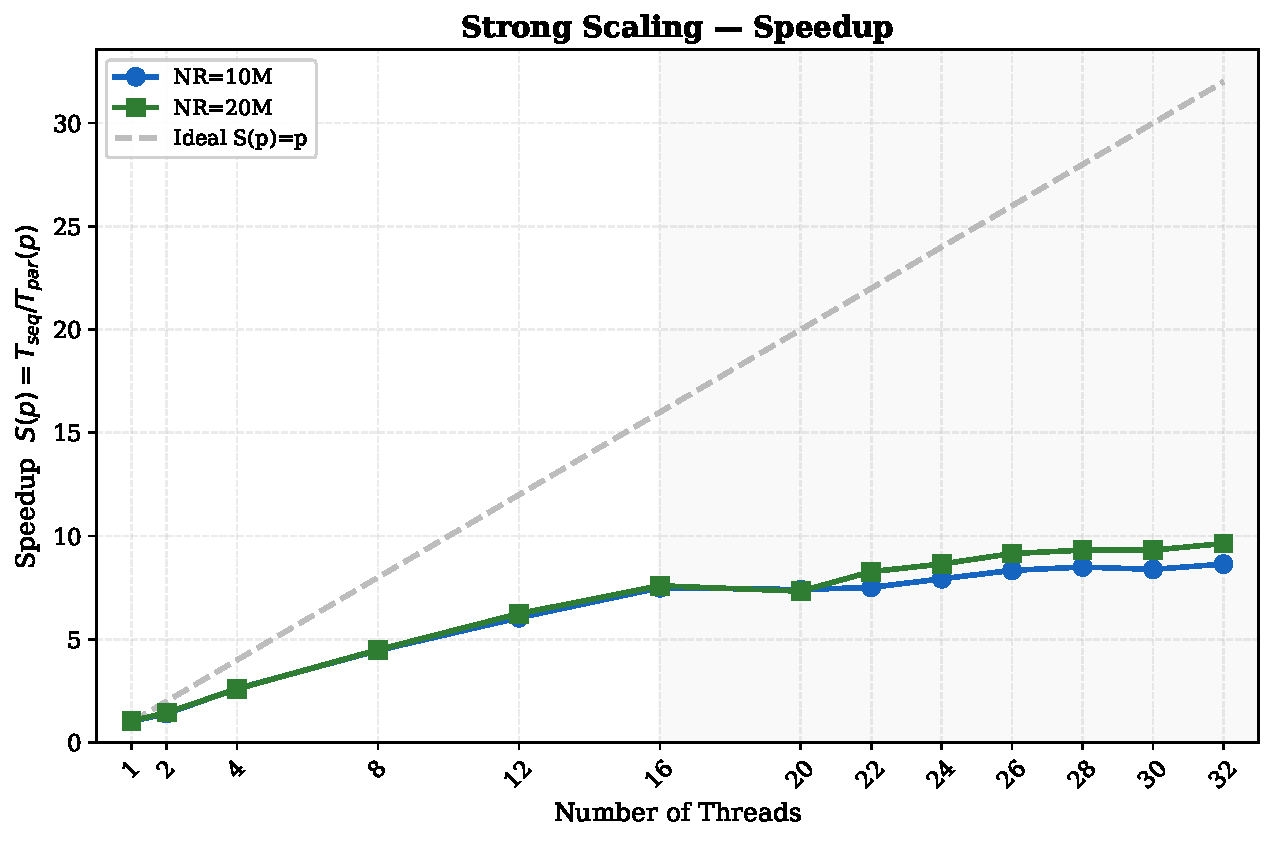
\includegraphics[width=\linewidth]{../results/plots/strong_speedup.pdf}
    \caption{Speedup $S(p) = T_\text{seq}/T_\text{par}(p)$.}
    \label{fig:strong_speedup}
  \end{subfigure}
  \hfill
  \begin{subfigure}[b]{0.49\textwidth}
    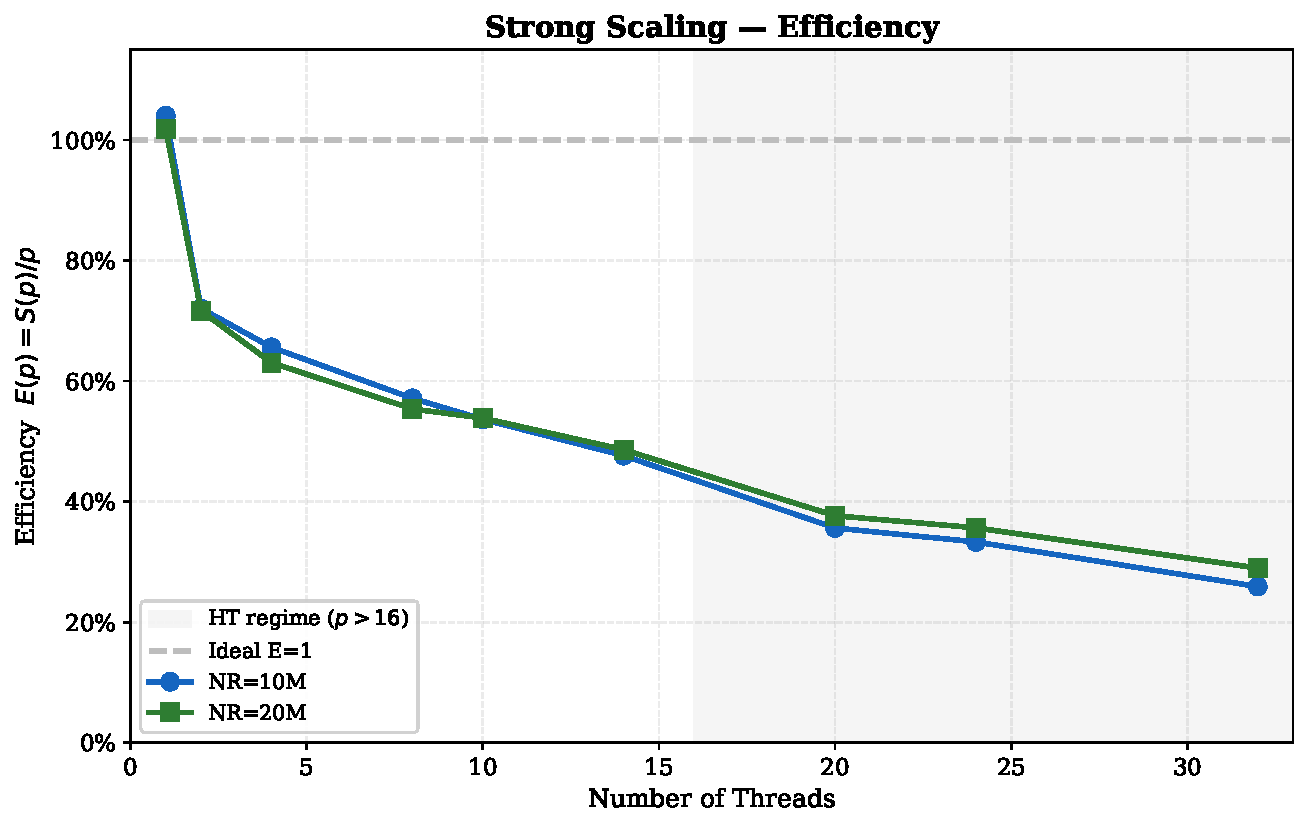
\includegraphics[width=\linewidth]{../results/plots/strong_efficiency.pdf}
    \caption{Efficienza $E(p) = S(p)/p$: dal 72\% a $p=2$ al 26\% a $p=32$. Righe grigie: thread HT ($p > 16$).}
    \label{fig:strong_eff}
  \end{subfigure}
  \caption{Strong scaling — i profili delle due dimensioni (NR=10M e NR=20M) coincidono quasi esattamente.}
\end{figure*}

\subsection*{Weak scaling}

Ogni thread elabora 1M record di $R$ (e 2M di $S$). WSE $= T(1)/T(p)$; il valore ideale è 1.0. Il punto di riferimento a $p=1$ ($\approx 78$\,ms su NR=1M) presenta overhead trascurabile dall'infrastruttura a barriera.

\begin{center}
\small
\begin{tabular}{@{}rrrr@{}}
\toprule
$p$ & NR & $T$ (ms) & WSE \\
\midrule
1  & 1M  &  78 & 1.00 \\
2  & 2M  & 106 & 0.74 \\
4  & 4M  & 112 & 0.70 \\
8  & 8M  & 131 & 0.60 \\
10 & 10M & 145 & 0.54 \\
14 & 14M & 155 & 0.51 \\
20 & 20M & 206 & 0.38 \\
\rowcolor{gray!15}
24 & 24M & 209 & 0.37 \\
\rowcolor{gray!15}
32 & 32M & 238 & 0.33 \\
\bottomrule
\end{tabular}
\end{center}

\begin{figure*}[t]
  \centering
  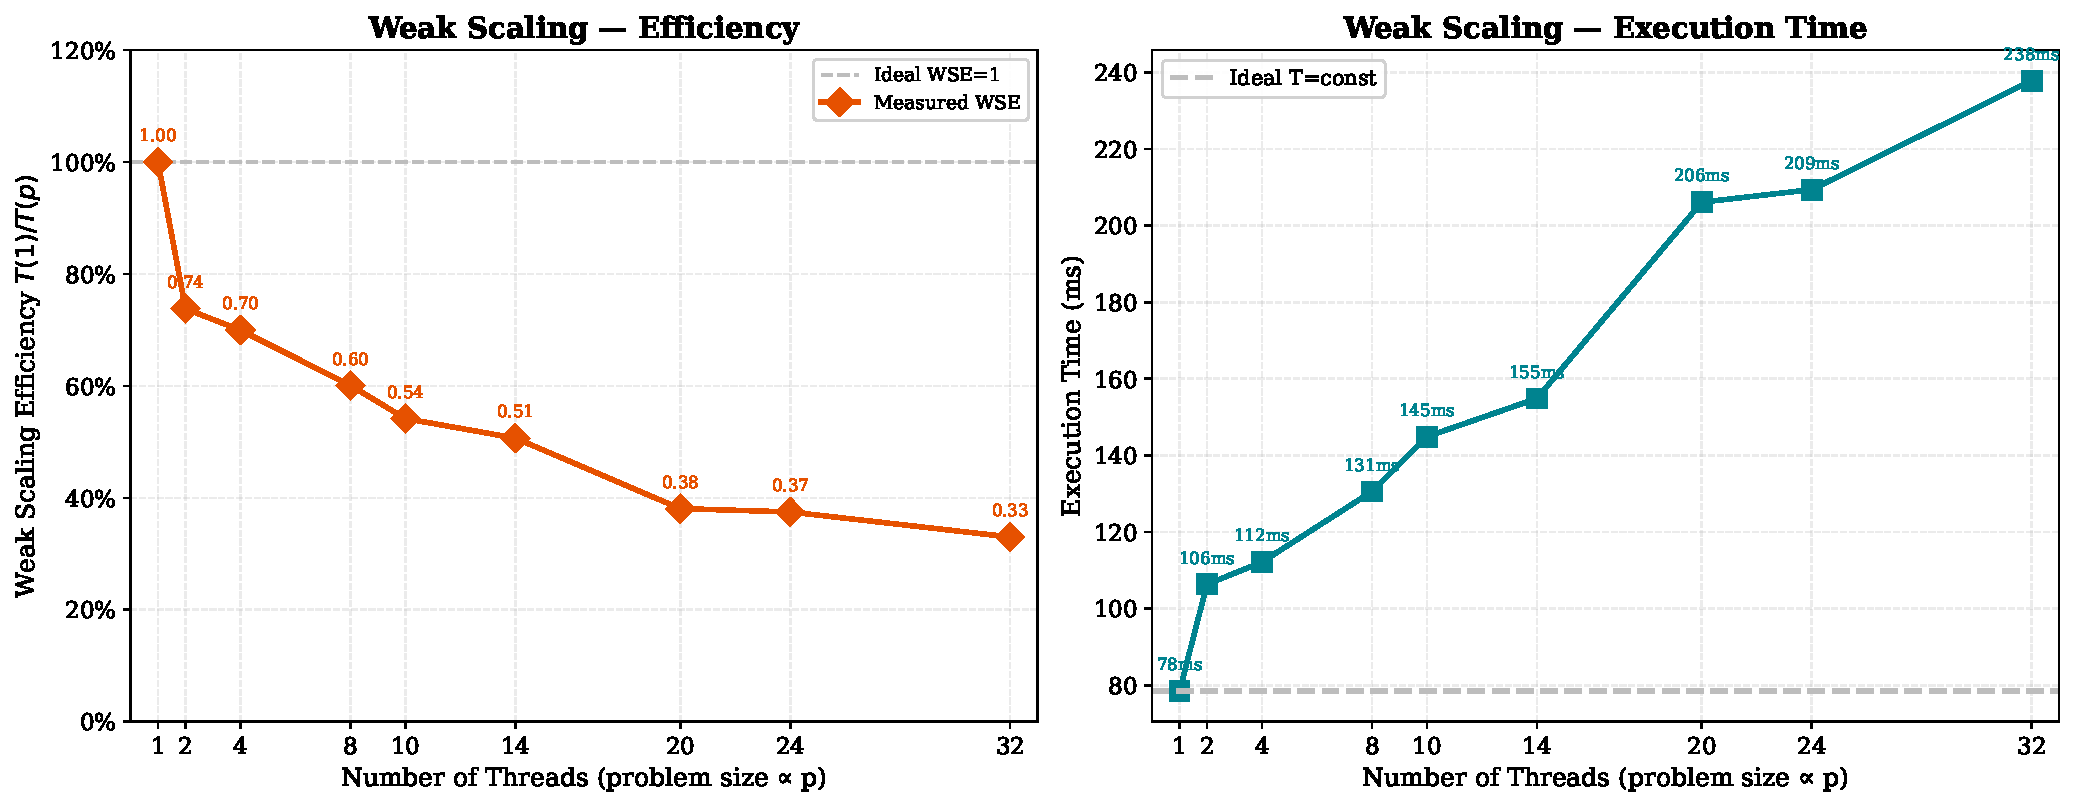
\includegraphics[width=0.85\textwidth]{../results/plots/weak_scaling.pdf}
  \caption{Weak scaling: efficienza (sinistra) e tempo assoluto (destra). La WSE decresce in modo monotono; il costo dominante è lo scatter, il cui pattern di scrittura random satura la banda DRAM al crescere della dimensione del problema (vedi §\ref{sec:discussion}).}
  \label{fig:weak}
\end{figure*}

\subsection*{Breakdown per fase}

\begin{center}
\small
\begin{tabular}{@{}lrrrr@{}}
\toprule
Fase & $T_\text{seq}$ & $S(20)$ & $S(24)$ & $S(32)$ \\
\midrule
Histogram R+S &  51\,ms &  2.4$\times$ &  3.2$\times$ &  2.7$\times$ \\
Scatter R+S   & 410\,ms &  9.7$\times$ & 11.3$\times$ & 13.7$\times$ \\
Join Local    & 300\,ms &  6.9$\times$ &  8.5$\times$ &  7.8$\times$ \\
\midrule
End-to-end    & 782\,ms &  7.1$\times$ &  8.0$\times$ &  8.3$\times$ \\
\bottomrule
\end{tabular}
\end{center}
{\footnotesize End-to-end include l'allocazione degli array partizionati ($\sim$480\,MB); i tempi di fase sono misurati dal timer interno della pipeline.}

\begin{figure}[h]
  \centering
  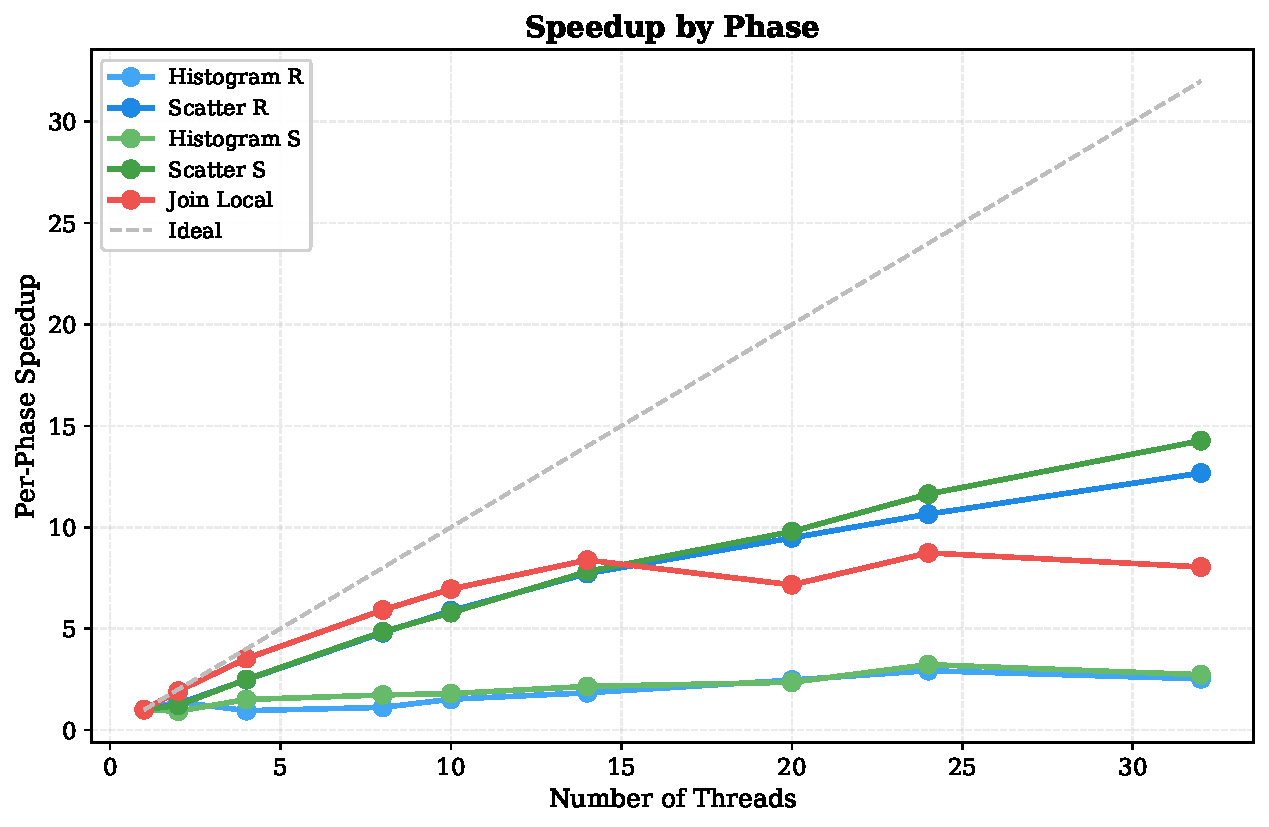
\includegraphics[width=\linewidth]{../results/plots/phase_speedup.pdf}
  \caption{Speedup per fase a 20 thread. Join Local e Scatter scalano bene; Histogram è limitato dalla banda di memoria.}
  \label{fig:phase_sp}
\end{figure}

% ===========================================================================
\section{Discussione}
\label{sec:discussion}
% ===========================================================================

\subsection*{Strong scaling e Legge di Amdahl}

Adattando la Legge di Amdahl $S(p) = 1/(f + (1{-}f)/p)$ all'intero dataset (inclusi $p=24,32$) si stima $f \approx 0{,}083$, con speedup massimo teorico $S_\infty = 1/f \approx 12{,}1\times$. Il picco misurato è $8{,}29\times$ (NR=10M, $p=32$) e $9{,}27\times$ (NR=20M, $p=32$). Il divario tra la previsione di Amdahl e il picco misurato è spiegato dalla saturazione della banda DRAM: al crescere dei thread, la banda di memoria è il vincolo dominante più della componente seriale.

L'efficienza scende dal 72\% a $p=2$ al 26\% a $p=32$ (NR=10M). Oltre $p=14$ core fisici il miglioramento del tempo end-to-end è inferiore al 15\% per raddoppio di thread, rendendo $p=14$--$20$ il punto di equilibrio pratico su questo hardware.

\textbf{Regime Hyper-Threading ($p = 20$--$32$).}
Il breakdown per fase rivela una divergenza controintuitiva oltre $p=16$: scatter continua a migliorare (R+S combinato: $9{,}7\times \to 13{,}7\times$ da $p=20$ a $p=32$) mentre join raggiunge il picco a $p=14$ ($8{,}1\times$) e poi regredisce a $6{,}9\times$ a $p=20$, recuperando a $7{,}8\times$ a $p=32$. Scatter è limitato dalla banda di memoria --- i thread HT aumentano il parallelismo di memoria (MLP), quindi i core logici aggiuntivi aiutano ancora. Join Local (lookup in \texttt{FlatCountMap}) è compute-bound: le coppie HT condividono le porte di esecuzione dello stesso core fisico, quindi i flussi di lookup concorrenti contendono per ALU e risorse L1/L2 anziché aggiungere capacità. Il risultato netto è un guadagno end-to-end moderato ($7{,}1\times \to 8{,}3\times$) nonostante il miglioramento dello scatter.

\begin{figure}[h]
  \centering
  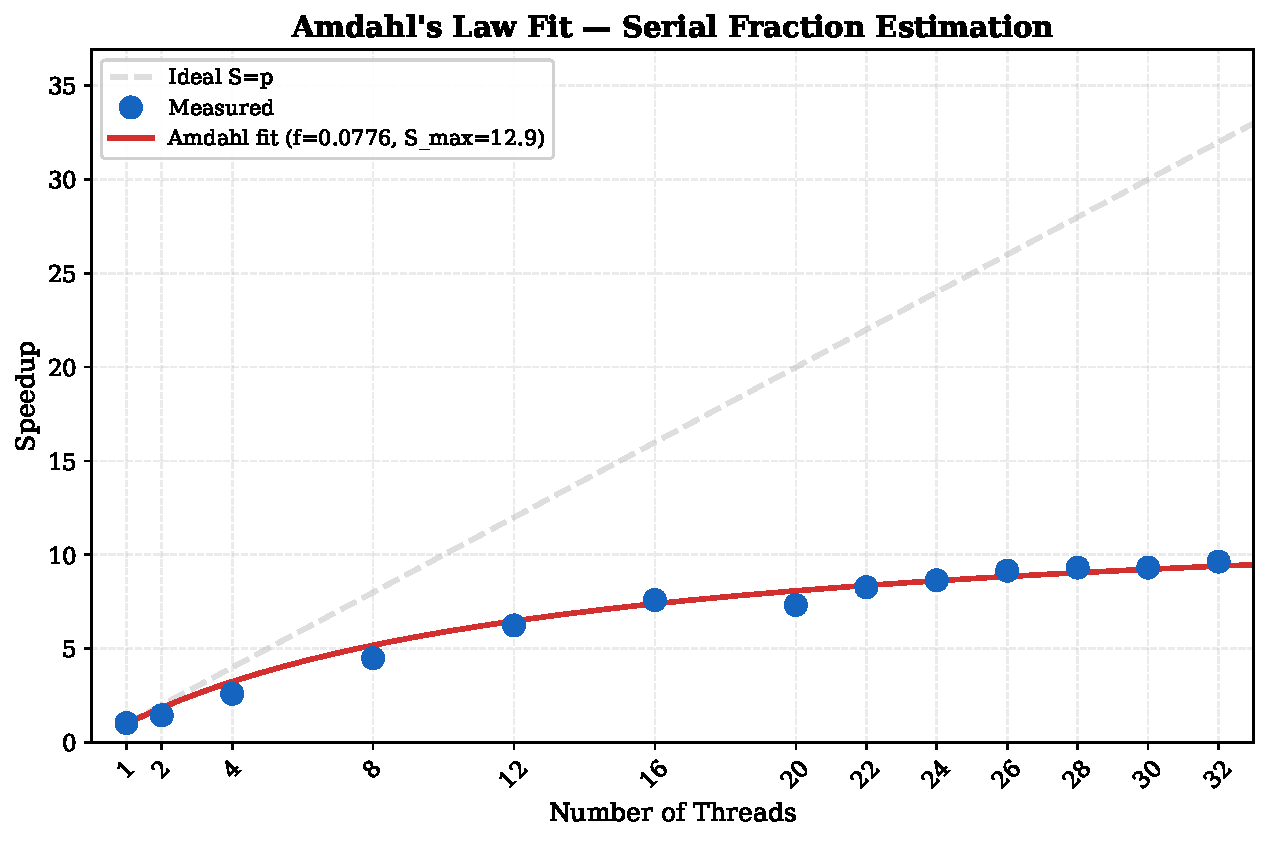
\includegraphics[width=\linewidth]{../results/plots/amdahl_fit.pdf}
  \caption{Fit della Legge di Amdahl (NR=20M). Frazione seriale stimata $f \approx 0{,}083$; speedup massimo teorico $S_\infty \approx 12{,}1\times$. Il picco misurato è inferiore alla previsione a causa della saturazione della banda di memoria.}
  \label{fig:amdahl}
\end{figure}

\subsection*{Weak scaling e interpretazione WSE}

Il binario parallelo a $p=1$ impiega $\approx 78$\,ms su NR=1M con overhead trascurabile dall'infrastruttura a barriera. La WSE $= T(1)/T(p)$ decresce in modo monotono: 0{,}74 a $p=2$, 0{,}54 a $p=10$, 0{,}33 a $p=32$.

La causa principale è lo scatter: al crescere della dimensione del problema proporzionalmente al numero di thread, il pattern di scrittura random genera un volume crescente di traffico DRAM che non può essere assorbito da più core (la banda è condivisa, non replicata). Histogram e join scalano leggermente meglio perché beneficiano di strutture private per thread (istogrammi locali) o rientrano nella capacità L3 aggregata. Il decadimento della WSE si accelera a $p>16$ a causa delle penalità NUMA: con due socket, una frazione crescente del working set di ciascun thread risiede sul nodo remoto.

\subsection*{Analisi per fase}

\textbf{Histogram (2.4--3.2$\times$ a $p=20$--$32$).}
Intensità aritmetica $I \approx 0{,}125$\,FLOP/byte: fase nella regione limitata dalla banda di memoria del modello Roofline. Gli istogrammi rappresentano solo il $\sim$7\% del tempo sequenziale, quindi la loro scarsa scalabilità influisce sul bound complessivo di meno del 5\% (Amdahl).

\textbf{Scatter (9.7--13.7$\times$ a $p=20$--$32$).}
Lo scatter domina ora il tempo sequenziale (54\%). Il design lock-free con offset pre-calcolati elimina ogni contesa; lo speedup è limitato solo dalla banda DRAM in scrittura. Il continuo miglioramento attraverso i thread HT (dal $9{,}7\times$ al $13{,}7\times$ da $p=20$ a $p=32$) conferma che questa fase beneficia dell'aumento del parallelismo di memoria.

\textbf{Join Local (picco $8{,}1\times$ a $p=14$, $7{,}8\times$ a $p=32$).}
Con $P=128$ e NR=10M, ogni partizione contiene $\approx 78$K record; la \texttt{FlatCountMap} occupa $\approx 4$\,MB (next-power-of-two sopra $2\times 78$K record: 262K slot $\times$ 16\,B), ben oltre la L2 (256\,KB) ma contenuta nella L3 condivisa da 20\,MB. L'assegnazione ciclica garantisce overhead di scheduling prossimo a zero per la hash uniforme Fibonacci. La fase scala quasi linearmente fino a $p=14$ ($8{,}1\times$); oltre $p=16$ i thread HT condividono le porte di esecuzione, causando la regressione descritta sopra.

\subsection*{Sensibilità al numero di partizioni}

Con $P \in [16, 4096]$ (a $p=20$, NR=10M), il tempo raggiunge il minimo a $P=512$--$1024$ ($\approx 86$\,ms), con una variazione complessiva di $< 1{,}6\times$. A $P=16$ ogni partizione contiene $\approx 625$K record e la \texttt{FlatCountMap} occupa $\approx 32$\,MB, spilling in DRAM. L'ottimo a $P=512$ corrisponde a $\approx 20$K record/partizione, con la hash table ($\approx 1$\,MB) che si adatta bene alla L3 condivisa da 20\,MB. Oltre $P=1024$ l'overhead dello scatter aumenta leggermente, portando il tempo a 94\,ms a $P=4096$. Un picco non monotono a $P=32$ (130\,ms, più lento di $P=16$) riflette una transizione di occupazione della cache tra i regimi DRAM-spill e L3-fit. L'ampio plateau attorno a $P \in [256, 1024]$ conferma che il numero di partizioni non è un parametro critico di tuning.

\begin{figure}[h]
  \centering
  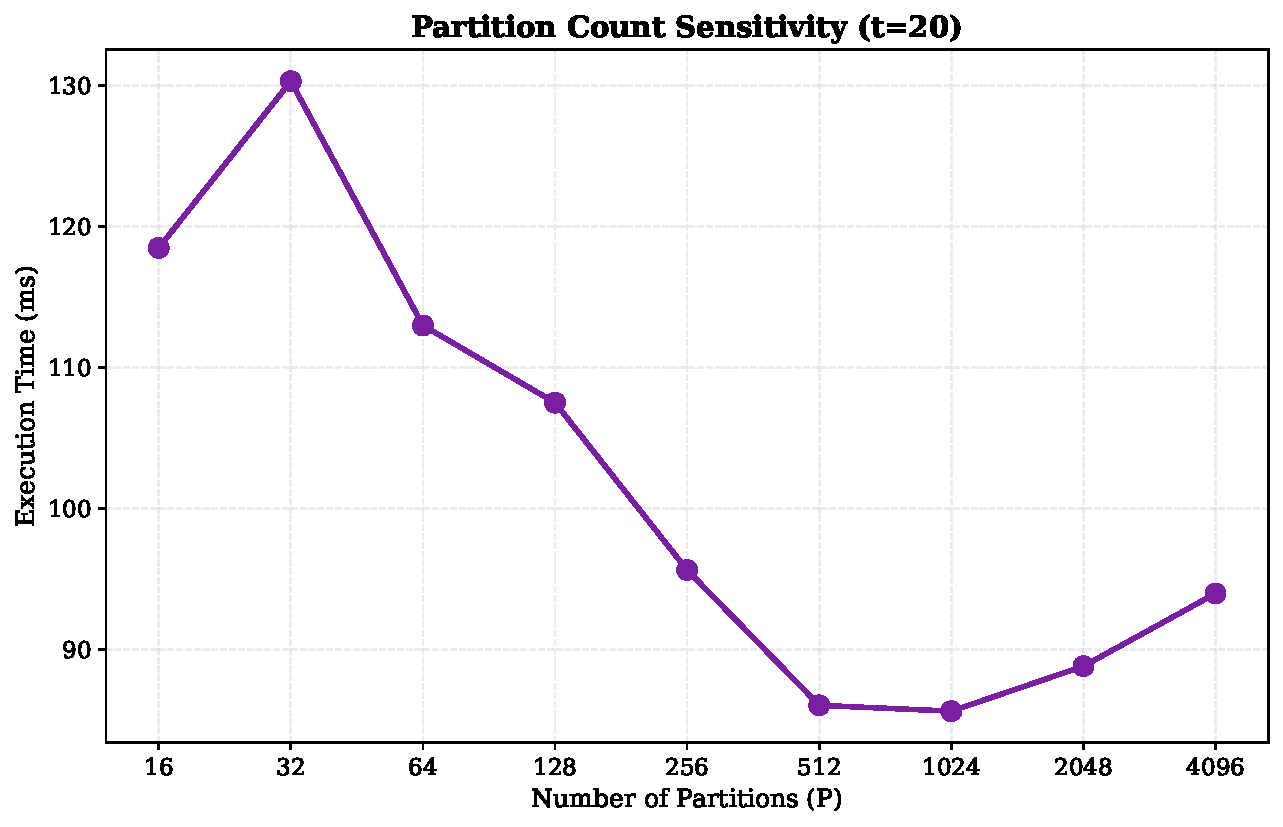
\includegraphics[width=\linewidth]{../results/plots/partition_sensitivity.pdf}
  \caption{Sensibilità al numero di partizioni ($p=20$, NR=10M). Minimo a $P=512$--$1024$; picco non monotono a $P=32$ dovuto a una transizione di occupazione della cache.}
  \label{fig:part_sens}
\end{figure}

\subsection*{Densità dei duplicati}

Il tempo sequenziale è essenzialmente costante per \texttt{max\_key} $\leq 1$M ($\approx 700$--$770$\,ms): con poche chiavi distinte la \texttt{FlatCountMap} per partizione ha pochi slot occupati e la maggior parte dei probe termina immediatamente. A \texttt{max\_key}=10M (chiavi quasi tutte distinte) la hash table è completamente popolata, aumentando il tempo sequenziale del $+31\%$ ($\approx 700$\,ms $\to$ 915\,ms) per maggiore pressione sulla L3 nella fase di join. Lo speedup parallelo rimane stabile su tutte le densità ($\approx 6{,}4$--$7{,}5\times$ a $p=20$), confermando che l'indipendenza delle partizioni non è influenzata dalla distribuzione delle chiavi.

\begin{figure}[h]
  \centering
  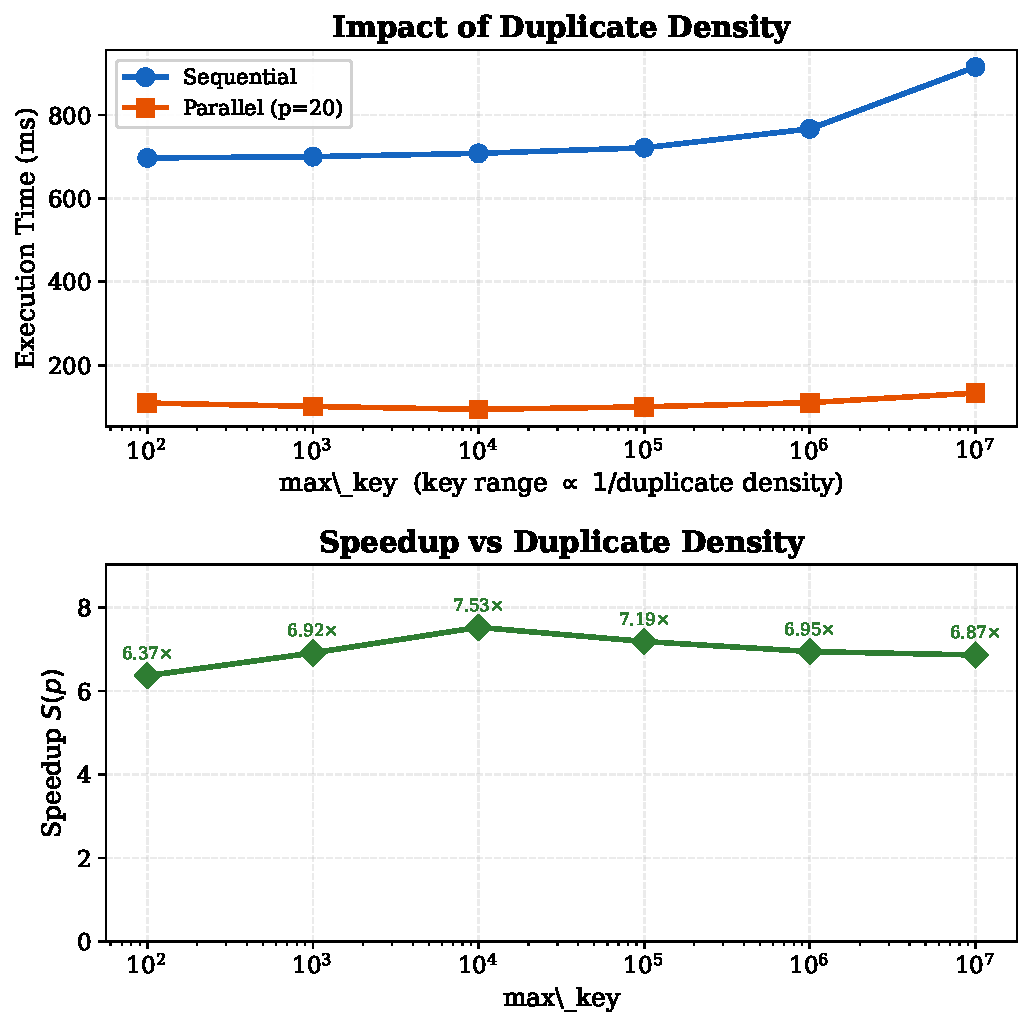
\includegraphics[width=\linewidth]{../results/plots/duplicate_density.pdf}
  \caption{Impatto della densità dei duplicati ($p=20$, NR=10M). Sinistra: tempi assoluti (seq e par). Destra: speedup vs.\ \texttt{max\_key}. Lo speedup rimane stabile ($6{,}4$--$7{,}5\times$) su tutte le densità.}
  \label{fig:dup}
\end{figure}

\end{document}
